\section{Introduction} \label{sec:intro}

% Shorter opening for IPEC.

The NP-hard \textsc{Odd Cycle Transversal} problem asks for a minimum vertex set whose removal from an undirected input graph~$G$ breaks all odd cycles, and thereby yields a bipartite graph. Finding odd cycle transversals has important applications, for example in computational biology~\cite{Huffner09,Wernicke14} and adiabatic quantum computing~\cite{GoodrichHS21,Goodrich18}. \textsc{Odd Cycle Transversal} parameterized by the desired solution size~$k$ has been studied intensively, leading to important advances such as \emph{iterative compression}~\cite{ReedSV04} and \emph{matroid-based kernelization}~\cite{KratschW14,KratschW20}. The randomized kernel due to Kratsch and Wahlstr\"{o}m~\cite[Lemma 7.11]{KratschW20} is a polynomial-time algorithm that reduces an $n$-vertex instance~$(G,k)$ of \textsc{Odd Cycle Transversal} to an instance~$(G',k')$ on~$\Oh((k \log k \log \log k)^3)$ vertices, that is equivalent to the input instance with probability at least~$2^{-n}$. Experiments with this matroid-based kernelization, however, show disappointing preprocessing results in practice~\cite{PilipczukZ18}. This formed one of the motivations for a recent line of research aimed at preprocessing that reduces the \emph{search space} explored by algorithms solving the reduced instance, rather than preprocessing aimed at reducing the \emph{encoding size} of the instance (which is captured by kernelization). To motivate our work, we present some background on this topic.

%\textsc{Odd Cycle Transversal} is a well-studied problem in (algorithmic) graph theory~\cite{Reed99,Thomassen01}. In its decision version it asks, given an undirected graph~$G$ and integer~$k$, whether there is a vertex set~$S \subseteq V(G)$ that intersects all \emph{odd} cycles of~$G$. Such a set is therefore called an \emph{odd cycle transversal} (OCT) in~$G$, and it is well-known that this ensures~$G - S$ is a bipartite graph. Finding odd cycle transversals has important applications, for example in computational biology~\cite{GoodrichHS21,Huffner09,Wernicke14}.\bmpr{Blair, do you have anything to add to the line about applications?} A simple reduction from \textsc{Vertex Cover} shows that \textsc{Odd Cycle Transversal} is NP-complete. The problem has therefore been subject of intensive study within the framework of parameterized complexity~\cite{CyganFKLMPPS15,DowneyF13}, which aims to develop exact algorithms in which the exponential dependence in the running time is confined to a \emph{parameter} of the input. Reed, Smith, and Vetta~\cite{ReedSV04} introduced the technique of \emph{iterative compression} to give a fixed-parameter tractable (FPT) algorithm for \textsc{Odd Cycle Transversal} parameterized by the size~$k$ of the desired solution, which runs in time~$3^k \cdot n^{\Oh(1)}$ on an $n$-vertex graph (cf.~\cite{Huffner09}). The current-fastest FPT algorithm~\cite{LokshtanovNRRS14} runs in time~$2.3146^k \cdot n^{\Oh(1)}$. It is based on a reduction to \textsc{Vertex Cover}, which is then solved by branching steps guided by its linear-programming relaxation~\cite{LokshtanovNRRS14}. 

%\textsc{Odd Cycle Transversal} has also been studied intensively from the perspective of \emph{kernelization}, which is a model for provably effective and efficient preprocessing. A \emph{kernelization} of size~$f \colon \mathbb{N} \to \mathbb{N}$ for a parameterized problem~$\mathcal{P}$ is a polynomial-time algorithm that reduces any parameterized instance~$(x,k)$ to an instance~$(x',k')$ with the same \textsc{yes/no} answer, such that~$|x'|, k' \leq f(k)$. It therefore guarantees that the size of the instance is reduced in terms of the complexity parameter~$k$. Despite its similary to the \textsc{Feedback Vertex Set} (FVS) problem on undirected graphs (which asks for a vertex set intersecting \emph{all} cycles, whose removal therefore yields a forest), developing a polynomial-size kernelization (a \emph{polynomial kernel}) for \textsc{Odd Cycle Transversal} proved to be much more difficult than for \textsc{Feedback Vertex Set}~\cite{BodlaenderD10,BurrageEFLMR06,Thomasse10,Iwata17}. Kratsch and Wahlstr\"{o}m introduced matroid-based techniques~\cite{KratschW14} to obtain a (randomized) polynomial kernel for \textsc{Odd Cycle Transversal}~\cite{KratschW20}. Their result~\cite[Lemma 7.11]{KratschW20} gives a randomized polynomial-time algorithm that reduces any instance~$(G,k)$ of \textsc{Odd Cycle Transversal} to an instance~$(G',k')$ on~$\Oh((k \log k \log \log k)^3)$ vertices, that is equivalent to the input instance with probability at least~$2^{-n}$. Experiments with this matroid-based kernelization show disappointing preprocessing results in practice, though~\cite{PilipczukZ18}. This formed one of the motivations for a recent line of research aimed at preprocessing that reduces the \emph{search space} explored by follow-up algorithms solving the reduced instance, rather than preprocessing aimed at reducing the \emph{encoding size} of the instance (which is captured by kernelization). To motivate our work, we present some background on this topic.

A \emph{kernelization} of size~$f \colon \mathbb{N} \to \mathbb{N}$ for a parameterized problem~$\mathcal{P}$ is a polynomial-time algorithm that reduces any parameterized instance~$(x,k)$ to an instance~$(x',k')$ with the same \textsc{yes/no} answer, such that~$|x'|, k' \leq f(k)$. It therefore guarantees that the size of the instance is reduced in terms of the complexity parameter~$k$. It does not directly ensure a reduction in the \emph{search space} of the follow-up algorithm that is employed to solve the reduced instance. Since the running times of FPT algorithms for the natural parameterization of \textsc{Odd Cycle Transversal}~\cite{Huffner09,ReedSV04,LokshtanovNRRS14} depend exponentially on the size of the sought solution, the size of the search space considered by such algorithms can be reduced significantly by a preprocessing step that finds some vertices~$S$ that belong to an optimal solution for the input graph~$G$: the search for a solution of size~$k$ on~$G$ then reduces to the search for a solution of size~$k-|S|$ on~$G-S$. Researchers therefore started to investigate in which situations an efficient preprocessing phase can guarantee finding part of an optimal solution. 

One line of inquiry in this direction aims at finding vertices that not only belong to an optimal solution, but are even required for building a $c$-approximate solution~\cite{BumpusJK22,JansenV24}; such vertices are called \emph{$c$-essential}. This has resulted in refined running time guarantees, showing that an optimal odd cycle transversal of size~$k$ can be found in time~$2.3146^{k - \ell} \cdot n^{\Oh(1)}$, where~$\ell$ is the number of vertices in the instance that are essential for making a 3-approximate solution~\cite{BumpusJK22}. Another line of research, more relevant to the subject of this paper, aims at finding vertices that belong to an optimal solution when there is a simple, locally verifiable certificate of the existence of an optimal solution containing them. So far, the latter direction has been explored for \textsc{Vertex Cover} (where a \emph{crown decomposition}~\cite{Abu-KhzamFLS07,Fellows03} forms such a certificate), and for the (undirected) \textsc{Feedback Vertex Set} problem (where an \emph{antler decomposition}~\cite{DonkersJ24}) forms such a certificate. 

\begin{figure*}[t]
  \centering

  \tikzstyle{plain} = [circle, fill=white, text=black, draw, thick, scale=1, minimum size=0.5cm, inner sep=1.5pt]
  \tikzstyle{small} = [circle, fill=white, text=black, draw, thick, scale=1, minimum size=0.2cm, inner sep=1.5pt]
  \tikzstyle{thickedge} = [line width=0.8mm]

  \begin{minipage}[m]{.32\textwidth}
      \vspace{0pt}
      \centering
      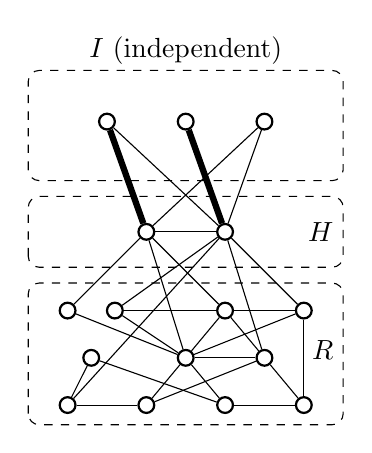
\begin{tikzpicture}
          % vertices
          \node[small] (r1) at (1, 1.8) {};
          \node[small] (r2) at (2, 1.8) {};
          \node[small] (r3) at (3, 1.8) {};
          \node[small] (r4) at (4, 1.8) {};

          \node[small] (r5) at (1.3, 2.4) {};
          \node[small] (r6) at (2.5, 2.4) {};
          \node[small] (r7) at (3.5, 2.4) {};

          \node[small] (r8) at (1, 3) {};
          \node[small] (r9) at (1.6, 3) {};
          \node[small] (r10) at (3, 3) {};
          \node[small] (r11) at (4, 3) {};

          \node[small] (c1) at (2, 4) {};
          \node[small] (c2) at (3, 4) {};

          \node[small] (b1) at (1.5, 5.4) {};
          \node[small] (b2) at (2.5, 5.4) {};
          \node[small] (b3) at (3.5, 5.4) {};

          % edges
          \draw (r1) -- (r2);
          \draw (r3) -- (r4);
          \draw (r1) -- (r5);
          \draw (r2) -- (r6);
          \draw (r2) -- (r7);
          \draw (r3) -- (r5);
          \draw (r3) -- (r6);
          \draw (r4) -- (r7);
          \draw (r6) -- (r7);
          \draw (r6) -- (r8);
          \draw (r6) -- (r9);
          \draw (r6) -- (r10);
          \draw (r6) -- (r11);
          \draw (r7) -- (r10);
          \draw (r4) -- (r11);
          \draw (r9) -- (r10);
          \draw (r10) -- (r11);

          \draw (r8) -- (c1);
          \draw (r6) -- (c1);
          \draw (r10) -- (c1);
          \draw (r7) -- (c2);
          \draw (r9) -- (c2);
          \draw (r11) -- (c2);
          \draw (r1) -- (c2);

          \draw (c1) -- (c2);
          \draw[thickedge] (c1) -- (b1);
          \draw (c1) -- (b3);
          \draw (c2) -- (b1);
          \draw[thickedge] (c2) -- (b2);
          \draw (c2) -- (b3);

          % annotation
          \draw[rounded corners, dashed] (0.5, 1.55) rectangle ++ (4, 1.8);
          \node[anchor=east] at (4.5, 2.5) {$R$};

          \draw[rounded corners, dashed] (0.5, 3.55) rectangle ++ (4, 0.9);
          \node[anchor=east] at (4.5, 4) {$H$};

          \draw[rounded corners, dashed] (0.5, 4.65) rectangle ++ (4, 1.4);
          \node[] at (2.5, 6.3) {$I$ (independent)};
      \end{tikzpicture}
  \end{minipage}
  \hfill
%
  \begin{minipage}[m]{.32\textwidth}
    \vspace{0pt}
    \centering
    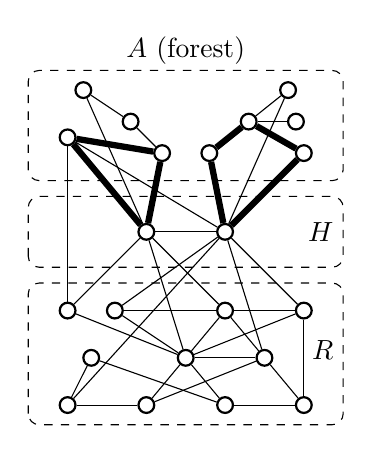
\begin{tikzpicture}
        % vertices
        \node[small] (r1) at (1, 1.8) {};
        \node[small] (r2) at (2, 1.8) {};
        \node[small] (r3) at (3, 1.8) {};
        \node[small] (r4) at (4, 1.8) {};

        \node[small] (r5) at (1.3, 2.4) {};
        \node[small] (r6) at (2.5, 2.4) {};
        \node[small] (r7) at (3.5, 2.4) {};

        \node[small] (r8) at (1, 3) {};
        \node[small] (r9) at (1.6, 3) {};
        \node[small] (r10) at (3, 3) {};
        \node[small] (r11) at (4, 3) {};

        \node[small] (c1) at (2, 4) {};
        \node[small] (c2) at (3, 4) {};

        \node[small] (b1) at (2.2, 5) {};
        \node[small] (b2) at (1.8, 5.4) {};
        \node[small] (b3) at (1.2, 5.8) {};
        \node[small] (b4) at (1, 5.2) {};

        \node[small] (b5) at (2.8, 5) {};
        \node[small] (b6) at (3.3, 5.4) {};
        \node[small] (b7) at (4, 5.0) {};
        \node[small] (b8) at (3.9, 5.4) {};
        \node[small] (b9) at (3.8, 5.8) {};

        % edges
        \draw (r1) -- (r2);
        \draw (r3) -- (r4);
        \draw (r1) -- (r5);
        \draw (r2) -- (r6);
        \draw (r2) -- (r7);
        \draw (r3) -- (r5);
        \draw (r3) -- (r6);
        \draw (r4) -- (r7);
        \draw (r6) -- (r7);
        \draw (r6) -- (r8);
        \draw (r6) -- (r9);
        \draw (r6) -- (r10);
        \draw (r6) -- (r11);
        \draw (r7) -- (r10);
        \draw (r4) -- (r11);
        \draw (r9) -- (r10);
        \draw (r10) -- (r11);

        \draw (r8) -- (c1);
        \draw (r6) -- (c1);
        \draw (r10) -- (c1);
        \draw (r7) -- (c2);
        \draw (r9) -- (c2);
        \draw (r11) -- (c2);
        \draw (r1) -- (c2);

        \draw (c1) -- (c2);
        \draw[thickedge] (c1) -- (b1);
        \draw (c1) -- (b3);
        \draw[thickedge] (c1) -- (b4);
        \draw (c2) -- (b4);
        \draw[thickedge] (c2) -- (b5);
        \draw[thickedge] (c2) -- (b7);
        \draw (c2) -- (b9);

        \draw (b1) -- (b2);
        \draw (b2) -- (b3);
        \draw[thickedge] (b1) -- (b4);
        \draw[thickedge] (b5) -- (b6);
        \draw[thickedge] (b6) -- (b7);
        \draw (b6) -- (b8);
        \draw (b6) -- (b9);

        \draw (b4) -- (r8);

        % annotation
        \draw[rounded corners, dashed] (0.5, 1.55) rectangle ++ (4, 1.8);
        \node[anchor=east] at (4.5, 2.5) {$R$};

        \draw[rounded corners, dashed] (0.5, 3.55) rectangle ++ (4, 0.9);
        \node[anchor=east] at (4.5, 4) {$H$};

        \draw[rounded corners, dashed] (0.5, 4.65) rectangle ++ (4, 1.4);
        \node[] at (2.5, 6.3) {$A$ (forest)};
      \end{tikzpicture}
  \end{minipage}
  \hfill
%
  \begin{minipage}[m]{.32\textwidth}
    \vspace{0pt}
    \centering
    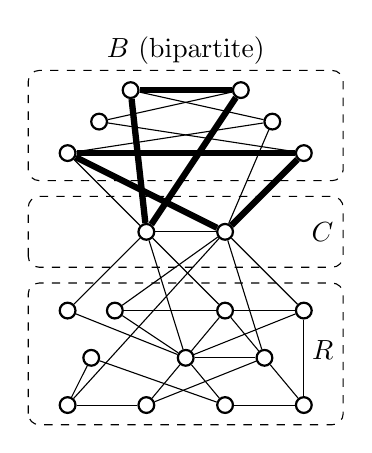
\begin{tikzpicture}
        % vertices
        \node[small] (r1) at (1, 1.8) {};
        \node[small] (r2) at (2, 1.8) {};
        \node[small] (r3) at (3, 1.8) {};
        \node[small] (r4) at (4, 1.8) {};

        \node[small] (r5) at (1.3, 2.4) {};
        \node[small] (r6) at (2.5, 2.4) {};
        \node[small] (r7) at (3.5, 2.4) {};

        \node[small] (r8) at (1, 3) {};
        \node[small] (r9) at (1.6, 3) {};
        \node[small] (r10) at (3, 3) {};
        \node[small] (r11) at (4, 3) {};

        \node[small] (c1) at (2, 4) {};
        \node[small] (c2) at (3, 4) {};

        \node[small] (b1) at (1, 5) {};
        \node[small] (b2) at (1.4, 5.4) {};
        \node[small] (b3) at (1.8, 5.8) {};

        \node[small] (b4) at (4, 5) {};
        \node[small] (b5) at (3.6, 5.4) {};
        \node[small] (b6) at (3.2, 5.8) {};

        % edges
        \draw (r1) -- (r2);
        \draw (r3) -- (r4);
        \draw (r1) -- (r5);
        \draw (r2) -- (r6);
        \draw (r2) -- (r7);
        \draw (r3) -- (r5);
        \draw (r3) -- (r6);
        \draw (r4) -- (r7);
        \draw (r6) -- (r7);
        \draw (r6) -- (r8);
        \draw (r6) -- (r9);
        \draw (r6) -- (r10);
        \draw (r6) -- (r11);
        \draw (r7) -- (r10);
        \draw (r4) -- (r11);
        \draw (r9) -- (r10);
        \draw (r10) -- (r11);

        \draw (r8) -- (c1);
        \draw (r6) -- (c1);
        \draw (r10) -- (c1);
        \draw (r7) -- (c2);
        \draw (r9) -- (c2);
        \draw (r11) -- (c2);
        \draw (r1) -- (c2);

        \draw (c1) -- (c2);
        \draw (c1) -- (b1);
        \draw[thickedge] (c1) -- (b3);
        \draw[thickedge] (c1) -- (b6);
        \draw[thickedge] (c2) -- (b1);
        \draw[thickedge] (c2) -- (b4);
        \draw (c2) -- (b5);

        \draw[thickedge] (b1) -- (b4);
        \draw (b1) -- (b5);
        \draw (b2) -- (b4);
        \draw (b2) -- (b6);
        \draw (b3) -- (b5);
        \draw[thickedge] (b3) -- (b6);

        % annotation
        \draw[rounded corners, dashed] (0.5, 1.55) rectangle ++ (4, 1.8);
        \node[anchor=east] at (4.5, 2.5) {$R$};

        \draw[rounded corners, dashed] (0.5, 3.55) rectangle ++ (4, 0.9);
        \node[anchor=east] at (4.5, 4) {$C$};

        \draw[rounded corners, dashed] (0.5, 4.65) rectangle ++ (4, 1.4);
        \node[] at (2.5, 6.3) {$B$ (bipartite)};
      \end{tikzpicture}
  \end{minipage}
%
  \caption{%
  Examples of crown decomposition (left),
  antler decomposition for \PrbFVSLong (middle) and 
  a tight OCC for \PrbOCTLong (right).
  Packings of forbidden subgraphs are highlighted in bold.
  }
  \label{fig:example}
\end{figure*}


A \emph{crown decomposition} (see \cref{fig:example}) of a graph~$G$ consists of a partition of its vertex set into three parts: the \emph{crown}~$I$ (which is required to be a non-empty independent set), the \emph{head}~$H$ (which is required to contain all neighbors of~$I$), and the \emph{remainder}~$R = V(G) \setminus (I \cup H)$, such that the graph~$G[I \cup H]$ contains a matching~$M$ of size~$|H|$. Since~$I$ is an independent set, this matching partners each vertex of~$H$ with a private neighbor in~$I$. The existence of a crown decomposition shows that there is an optimal vertex cover (a minimum-size vertex set intersecting all edges) that contains all vertices of~$H$ and none of~$I$: any vertex cover contains at least~$|M| = |H|$ vertices from~$I \cup H$ to cover the matching~$M$, while~$H$ covers all the edges of~$G$ that can be covered by selecting vertices from~$I \cup H$. Hence a crown decomposition forms a polynomial-time verifiable certificate that there is an optimal vertex cover containing all vertices of~$H$. It facilitates a reduction in search space for \textsc{Vertex Cover}: graph~$G$ has a vertex cover of size~$k$ if and only if~$G - (I \cup H)$ has one of size~$k - |H|$. A crown decomposition can be found in polynomial time if it exists, which yields a powerful reduction rule for \textsc{Vertex Cover}~\cite{Abu-KhzamFLS07}.

% \bmpr{To be discussed: whether we want to require an antler to be non-empty, or to use the adjective everywhere.}

Inspired by this decomposition for \textsc{Vertex Cover}, Donkers and Jansen~\cite{DonkersJ24} introduced the notion of an \emph{antler decomposition} of a graph~$G$. It is a partition of the vertex set into three parts: the \emph{antler}~$A$ (which is required to induce a non-empty acyclic graph), the \emph{head}~$H$ (which is required to contain \emph{almost} all neighbors of~$A$: for each tree~$T$ in the forest~$G[A]$, there is at most one edge that connects~$T$ to a vertex outside~$H$), and the \emph{remainder}~$R = V(G) \setminus (A \cup H)$, while satisfying an additional condition in terms of an integer~$z$ that represents the \emph{order} of the antler decomposition. In its simplest form for~$z=1$ (we discuss~$z > 1$ later), the additional condition says that the graph~$G[A \cup H]$ should contain~$|H|$ vertex-disjoint cycles. Since~$G[A]$ is acyclic, each of these cycles contains exactly one vertex of~$H$. They certify that any feedback vertex set of~$G$ contains at least~$|H|$ vertices from~$A \cup H$. Since~$A$ induces an acyclic graph, and all cycles in~$G$ that enter a tree~$T$ of~$G[A]$ from~$R$ must leave~$A$ from~$H$, the set~$H$ intersects all cycles of~$G$ that contain a vertex of~$A \cup H$. Hence there is an optimal feedback vertex set containing~$H$. By finding an antler decomposition we can therefore reduce the problem of finding a size-$k$ solution in~$G$ to finding a size-($k - |H|$) solution in~$G - (A \cup H)$, and therefore reduce the search space for algorithms parameterized by solution size.

Donkers and Jansen proved that, assuming $\mathsf{P} \neq \mathsf{NP}$, there unfortunately is no polynomial-time algorithm to find an antler decomposition if one exists~\cite[Theorem 3.4]{DonkersJ24}. However, they gave a \emph{fixed-parameter tractable} preprocessing algorithm, parameterized by the size of the head. There is an algorithm that, given a graph~$G$ and integer~$k$ such that~$G$ contains an antler decomposition~$(A,H,R)$ with~$|H| = k$, runs in time~$2^{\Oh(k^5)} \cdot n^{\Oh(1)}$ and outputs a set of at least~$k$ vertices that belong to an optimal feedback vertex set. For each fixed value of~$k$, this yields a preprocessing algorithm to detect vertices that belong to an optimal solution if there is a simple certificate of their membership in an optimal solution.

In fact, Donkers and Jansen gave a more general algorithm; this is where $z$-antlers for~$z > 1$ make an appearance. Recall that for a $1$-antler decomposition~$(A,H,R)$ of a graph~$G$, the graph~$G[A \cup H]$ must contain a collection~$\mathcal{C}$ of~$|H|$ vertex-disjoint cycles. These cycles certify that the set~$H$ is an optimal feedback vertex set in the graph~$G[A \cup H]$. In fact, the feedback vertex set~$H$ in~$G[A \cup H]$ is already optimal for the subgraph~$\mathcal{C} \subseteq G[A \cup H]$, and that subgraph~$\mathcal{C}$ is structurally simple because each of its connected components (which is a cycle) has a feedback vertex set of size~$z=1$. This motivates the following definition of a $z$-antler decomposition for~$z>1$: the set~$H$ should be an optimal feedback vertex set for the subgraph~$G[A \cup H]$, and moreover, there should be a subgraph~$\mathcal{C}_z \subseteq G[A \cup H]$ such that (1)~$H$ is an optimal feedback vertex set in~$\mathcal{C}_z$, and (2)~each connected component of~$\mathcal{C}_z$ has a feedback vertex set of size at most~$z$. So for a $z$-antler decomposition~$(A,H,R)$ of a graph~$G$, there is a certificate that~$H$ is part of an optimal solution in the overall graph~$G$ that consists of the decomposition together with the subgraph~$\mathcal{C}_z \subseteq G[A \cup H]$ for which~$H$ is an optimal solution. The complexity of verifying this certificate scales with~$z$: it comes down to verifying that~$H \cap V(C)$ is indeed an optimal feedback vertex set of size at most~$z$ for each connected component of the subgraph~$\mathcal{C}_z$. Donkers and Jansen presented an algorithm that, given integers~$k \geq z \geq 0$ and a graph~$G$ that contains a $z$-antler decomposition whose head has size~$k$, outputs a set of at least~$k$ vertices that belongs to an optimal feedback vertex set in time~$2^{\Oh(k^5 z^2)} n^{\Oh(z)}$. For each fixed choice of~$k$ and~$z$, this gives a reduction rule (that can potentially be applied numerous times on an instance) to reduce the search space if the preconditions are met.

\subparagraph*{Our contribution} We investigate search-space reduction for \textsc{Odd Cycle Transversal}, thereby continuing the line of research proposed by Donkers and Jansen~\cite{DonkersJ24}. We introduce the notion of \emph{tight odd cycle cuts} to provide efficiently verifiable witnesses that a certain vertex set belongs to an optimal odd cycle transversal, and present algorithms to find vertices that belong to an optimal solution in inputs that admit such witnesses.

To be able to state our main result, we introduce the corresponding terminology. An \emph{odd cycle cut} (OCC) in an undirected graph~$G$ is a partition of its vertex set into three parts: the bipartite part~$B$ (which is required to induce a bipartite subgraph of~$G$), the cut part~$C$ (which is required to contain all neighbors of~$B$), and the rest~$R = V(G) \setminus (B \cup C)$. An odd cycle cut is called \emph{tight} if the set~$C$ forms an optimal odd cycle transversal for the graph~$G[B \cup C]$. In this case, it is easy to see that there is an optimal odd cycle transversal in~$G$ that contains all vertices of~$C$, since all odd cycles through~$B$ are intersected by~$C$. A tight OCC~$(B,C,R)$ has \emph{order~$z$} if there is a subgraph~$\mathcal{C}_z$ of~$G[B \cup C]$ for which~$C$ is an optimal odd cycle transversal, and for which each connected component of~$\mathcal{C}_z$ has an odd cycle transversal of size at most~$z$. This means that for~$z=1$, if there is such a subgraph~$\mathcal{C}_z \subseteq G[B \cup C]$, then there is one consisting of~$|C|$ vertex-disjoint odd cycles. We use the term $z$-tight OCC to refer to a tight OCC of order~$z$. Our notion of $z$-tight OCCs forms an analogue of $z$-antler decompositions. Note that the requirement that~$C$ contains \emph{all} neighbors of~$B$ is slightly more restrictive than in the \textsc{Feedback Vertex Set} case. We need this restriction for technical reasons, but discuss potential relaxations in \cref{sec:conclusion}.

Similarly to the setting of $z$-antlers for \textsc{Feedback Vertex Set}, assuming $\mathsf{P} \neq \mathsf{NP}$ there is no polynomial-time algorithm that always finds a tight OCC in a graph if one exists; not even in the case~$z=1$ (\cref{thm:1tight:occ:nphard}). We therefore develop algorithms that are efficient for small~$k$ and~$z$. The following theorem captures our main result, which is an OCT-analogue of the antler-based preprocessing algorithm for FVS. The \emph{width} of an OCC~$(B,C,R)$ is defined as~$|C|$. Our theorem shows that for constant~$z$ we can efficiently find~$k$ vertices that belong to an optimal solution, if there is a $z$-tight OCC of width~$k$.
%
\begin{restatable}{theorem}{thmMain}
  \label{thm:main}
  There is a deterministic algorithm that, given a graph $G$ and integers $k \geq z \geq 0$, runs in $2^{\Oh(k^{33} z^2)}\cdot n^{\Oh{(z)}}$ time and either outputs at least $k$ vertices that belong to an optimal solution for \PrbOCTLong, or concludes that $G$ does not contain a \zocc of width $k$.
\end{restatable}
%
One may wonder whether it is feasible to have more control over the output, by having the algorithm output a $z$-tight OCC~$(B,C,R)$ of width~$k$, if one exists. However, a small adaptation of a W[1]-hardness proof for antlers~\cite[Theorem 3.7]{DonkersJ24} shows (\cref{thm:tightocc:w1hard}) that the corresponding algorithmic task is W[1]-hard even for~$z=1$. This explains why the algorithm outputs a vertex set that belongs to an optimal solution, rather than a $z$-tight OCC.

In terms of techniques, our algorithm combines insights from the previous work on antlers~\cite{DonkersJ24} with ideas in the representative-set based kernelization~\cite{KratschW20} for \textsc{Odd Cycle Transversal}. The global idea behind the algorithm is to repeatedly simplify the graph, while preserving the structure of $z$-tight OCCs, to arrive at the following favorable situation: if there was a $z$-tight OCC of width~$k$ in the input, then the reduced graph has a $z$-tight OCC~$(B,C,R)$ of the same width that satisfies~$|B| \in k^{\Oh(1)}$. At that point, we can use color coding with a set of~$k^{\Oh(1)}$ colors to ensure that the structure~$B \cup C$ gets colored in a way that makes it tractable to identify it. The simplification steps on the graph are inspired by the kernelization for \textsc{Odd Cycle Transversal} and involve the computation of a \emph{cut covering set} of size~$k^{\Oh(1)}$ that contains a minimum three-way~$\{X,Y,Z\}$-separator
% \rfar{In our application, we specifically construct a cut covering set that contains minimum \emph{3-way} separators. Should the text (which mentions $(X, Y)$-separators) be updated to reflect this? \bmp{Done.}}
for all possible choices of sets~$\{X,Y,Z\}$ drawn from a terminal set~$T$ of size~$k^{\Oh(1)}$. The existence of such sets follows from the matroid-based tools of Kratsch and Wahlstr\"{o}m~\cite{KratschW20}. We can avoid the randomization incurred by their polynomial-time algorithm by computing a cut covering set in~$2^{\Oh(k)} \cdot n^{\Oh(1)}$ time deterministically. Compared to the kernelization for \textsc{Odd Cycle Transversal}, a significant additional challenge we face in this setting is that the size of OCTs in the graph can be arbitrarily large in terms of the parameter~$k$. Our algorithm is looking for a \emph{small} region of the graph in which a vertex set exists with a simple certificate for its membership in an optimal solution; it cannot afford to learn the structure of global OCTs in the graph. This local perspective poses a challenge when repeatedly simplifying the graph: we not only have to be careful how these operations affect the total solution size in~$G$, but also how these modifications affect the existence of simple certificates for membership in an optimal solution. This is why our reduction step works with three-way separators, rather than the two-way separators that suffice to solve or kernelize OCT.

\subparagraph*{Organization} The remainder of this work is organized as follows. The first twelve pages of the manuscript present the key statements and ideas. For statements marked $(\bigstar$), the proof is deferred to a later section for readability. After presenting preliminaries on graphs in \cref{sec:prelims}, we define (tight) OCCs in \cref{sec:oct:cut} and explore some of their properties. In \cref{sec:find:occs} we show how color coding can be used to find an OCC whose bipartite part is connected and significantly larger than its cut. Given such an OCC, we show in \cref{sec:reduce:occ} how to simplify the graph while preserving the essential structure of odd cycles in the graph. This leads to an algorithm that finds vertices belonging to an optimal solution the presence of a tight OCC in \cref{sec:tight:occs}. Sections~\ref{sec:more:prelims}--\ref{sec:tight:occs-proof} contain the deferred proofs. In \cref{sec:hardness} we give the hardness proofs mentioned above. Finally, we conclude in \cref{sec:conclusion}. 
